\begin{figure}[!h]
    \centering
    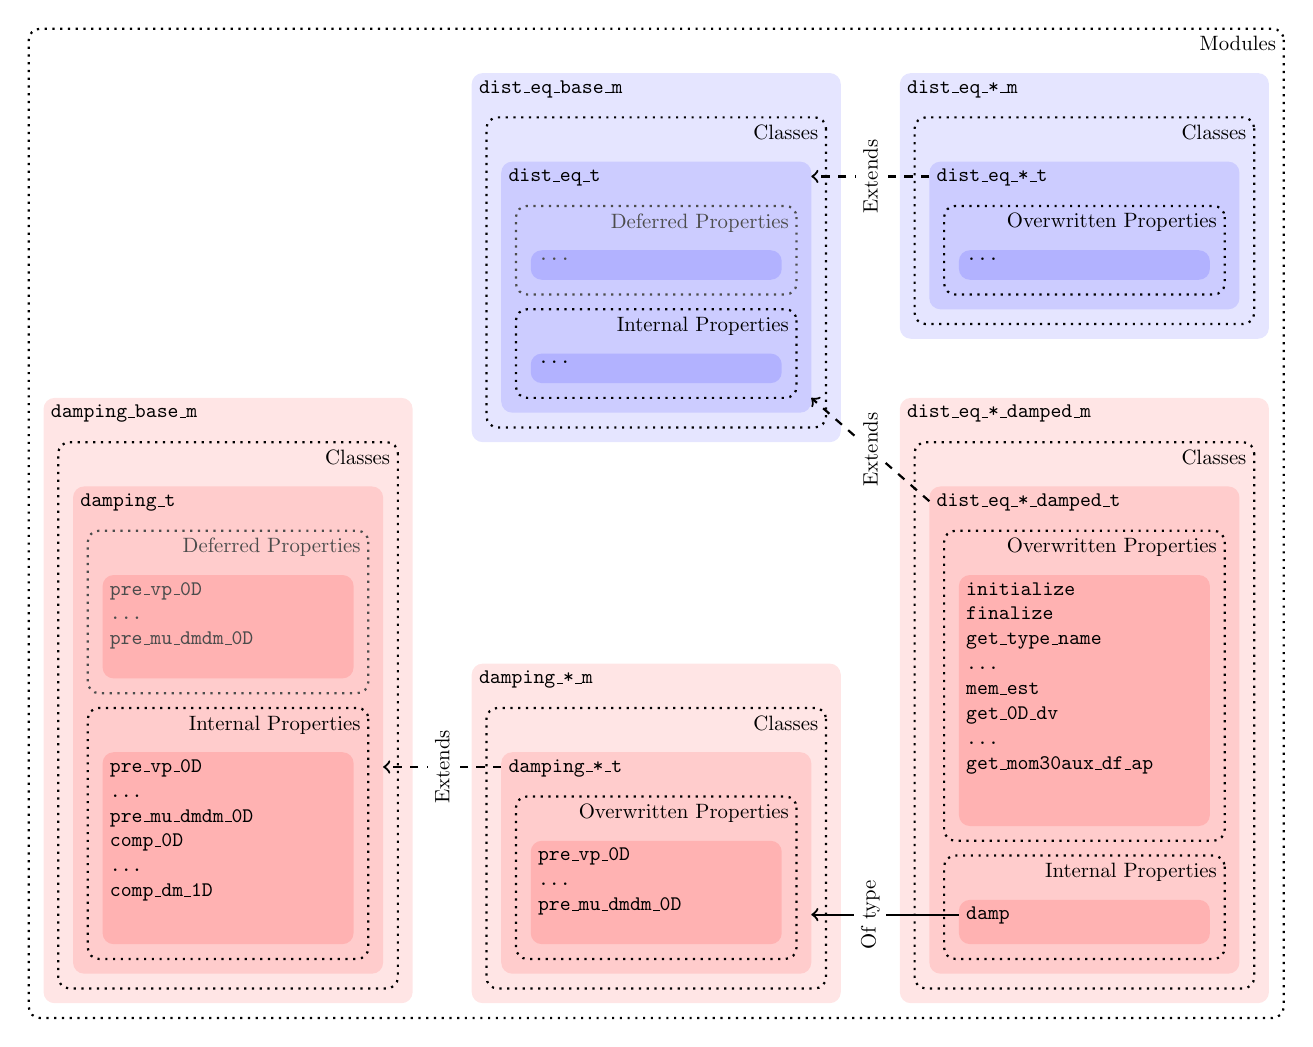
\begin{tikzpicture}[scale = 0.75, every node/.style = {scale = 0.75}, every text node part/.style = {align = left}]
        \draw[rounded corners, dotted, thick]
            (13.75, 0.75) node[below left] {Modules}
            rectangle
            (-7.5, -16);
            \fill[rounded corners, fill = blue!10]
                (0, 0) node[below right] {\tt dist\_eq\_base\_m}
                rectangle
                (6.25, -6.25);
                \draw[rounded corners, dotted, thick]
                    (6, -0.75) node[below left] {Classes}
                    rectangle
                    (0.25, -6);
                    \fill[rounded corners, fill = blue!20]
                        (0.5, -1.5) node[below right] {\tt dist\_eq\_t}
                        rectangle
                        (5.75, -5.75);
                        \draw[rounded corners, dotted, thick, dotted, black!70]
                            (5.5, -2.25) node[below left] {Deferred Properties}
                            rectangle
                            (0.75, -3.75);
                            \fill[rounded corners, fill = blue!30]
                                (1, -3) node[below right] {}
                                rectangle
                                (5.25, -3.5);
                            \node[black!70] at (1, -3) [below right] {
                                    {\tt ...}
                                };
                        \draw[rounded corners, dotted, thick]
                            (5.5, -4) node[below left] {Internal Properties}
                            rectangle
                            (0.75, -5.5);
                            \fill[rounded corners, fill = blue!30]
                                (1, -4.75) node[below right] {}
                                rectangle
                                (5.25, -5.25);
                            \node at (1, -4.75) [below right] {
                                    {\tt ...}
                                };
            \fill[rounded corners, fill = blue!10]
                (7.25, 0) node[below right] {\tt dist\_eq\_*\_m}
                rectangle
                (13.5, -4.5);
                \draw[rounded corners, dotted, thick]
                    (13.25, -0.75) node[below left] {Classes}
                    rectangle
                    (7.5, -4.25);
                    \fill[rounded corners, fill = blue!20]
                        (7.75, -1.5) node[below right] {\tt dist\_eq\_*\_t}
                        rectangle
                        (13, -4);
                        \draw[rounded corners, dotted, thick]
                            (12.75, -2.25) node[below left] {Overwritten Properties}
                            rectangle
                            (8, -3.75);
                            \fill[rounded corners, fill = blue!30]
                                (8.25, -3) node[below right] {}
                                rectangle
                                (12.5, -3.5);
                            \node at (8.25, -3) [below right] {
                                    {\tt ...}
                                };
            \fill[rounded corners, fill = red!10]
                (-7.25, -5.5) node[below right] {\tt damping\_base\_m}
                rectangle
                (-1, -15.75);
                \draw[rounded corners, dotted, thick]
                    (-1.25, -6.25) node[below left] {Classes}
                    rectangle
                    (-7, -15.5);
                    \fill[rounded corners, fill = red!20]
                        (-6.75, -7) node[below right] {\tt damping\_t}
                        rectangle
                        (-1.5, -15.25);
                        \draw[rounded corners, dotted, thick, dotted, black!70]
                            (-1.75, -7.75) node[below left] {Deferred Properties}
                            rectangle
                            (-6.5, -10.5);
                            \fill[rounded corners, fill = red!30]
                                (-6.25, -8.5) node[below right] {}
                                rectangle
                                (-2, -10.25);
                            \node[black!70] at (-6.25, -8.5) [below right] {
                                    {\tt pre\_vp\_0D} \\
                                    {\tt ...} \\
                                    {\tt pre\_mu\_dmdm\_0D}
                                };
                        \draw[rounded corners, dotted, thick]
                            (-1.75, -10.75) node[below left] {Internal Properties}
                            rectangle
                            (-6.5, -15);
                            \fill[rounded corners, fill = red!30]
                                (-6.25, -11.5) node[below right] {}
                                rectangle
                                (-2, -14.75);
                            \node at (-6.25, -11.5) [below right] {
                                    {\tt pre\_vp\_0D} \\
                                    {\tt ...} \\
                                    {\tt pre\_mu\_dmdm\_0D}  \\
                                    {\tt comp\_0D} \\
                                    {\tt ...} \\
                                    {\tt comp\_dm\_1D}
                                };
            \fill[rounded corners, fill = red!10]
                (0, -10) node[below right] {\tt damping\_*\_m}
                rectangle
                (6.25, -15.75);
                \draw[rounded corners, dotted, thick]
                    (6, -10.75) node[below left] {Classes}
                    rectangle
                    (0.25, -15.5);
                    \fill[rounded corners, fill = red!20]
                        (0.5, -11.5) node[below right] {\tt damping\_*\_t}
                        rectangle
                        (5.75, -15.25);
                        \draw[rounded corners, dotted, thick]
                            (5.5, -12.25) node[below left] {Overwritten Properties}
                            rectangle
                            (0.75, -15);
                            \fill[rounded corners, fill = red!30]
                                (1, -13) node[below right] {}
                                rectangle
                                (5.25, -14.75);
                            \node at (1, -13) [below right] {
                                    {\tt pre\_vp\_0D} \\
                                    {\tt ...} \\
                                    {\tt pre\_mu\_dmdm\_0D}
                                };
            \fill[rounded corners, fill = red!10]
                (7.25, -5.5) node[below right] {\tt dist\_eq\_*\_damped\_m}
                rectangle
                (13.5, -15.75);
                \draw[rounded corners, dotted, thick]
                    (13.25, -6.25) node[below left] {Classes}
                    rectangle
                    (7.5, -15.5);
                    \fill[rounded corners, fill = red!20]
                        (7.75, -7) node[below right] {\tt dist\_eq\_*\_damped\_t}
                        rectangle
                        (13, -15.25);
                        \draw[rounded corners, dotted, thick]
                            (12.75, -7.75) node[below left] {Overwritten Properties}
                            rectangle
                            (8, -13);
                            \fill[rounded corners, fill = red!30]
                                (8.25, -8.5) node[below right] {}
                                rectangle
                                (12.5, -12.75);
                            \node at (8.25, -8.5) [below right] {
                                    {\tt initialize} \\
                                    {\tt finalize} \\
                                    {\tt get\_type\_name} \\
                                    {\tt ...} \\
                                    {\tt mem\_est} \\
                                    {\tt get\_0D\_dv} \\
                                    {\tt ...} \\
                                    {\tt get\_mom30aux\_df\_ap}
                                };
                        \draw[rounded corners, dotted, thick]
                            (12.75, -13.25) node[below left] {Internal Properties}
                            rectangle
                            (8, -15);
                            \fill[rounded corners, fill = red!30]
                                (8.25, -14) node[below right] {}
                                rectangle
                                (12.5, -14.75);
                            \node at (8.25, -14) [below right] {
                                    {\tt damp}
                                };
        \draw[->, thick, dashed]
            (7.75, -1.75) -- (5.75, -1.75)
            node[midway, rotate = 90, fill = white] {Extends};
        \draw[->, thick, dashed]
            (7.75, -7.25) -- (5.75, -5.5)
            node[midway, rotate = 90, fill = white] {Extends};
        \draw[->, thick, dashed]
            (0.5, -11.75) -- (-1.5, -11.75)
            node[midway, rotate = 90, fill = white] {Extends};
        \draw[->, thick]
            (8.25, -14.25) -- (5.75, -14.25);
            \node[rotate = 90, fill = white] at (6.75, -14.25) {Of type};
    \end{tikzpicture}
    \caption{{\tt GENE} equilibrium distribution class structure \emph{after} addition of damping modules. Base modules marked in {\color{blue!90} blue}, additions marked in {\color{red!90} red}.}
    \label{class structure after damping}
\end{figure}